% !TEX root = ../../../main.tex

\begin{figure}[!htbp]
  \centering
  \begin{subfigure}[b]{0.4\textwidth}
    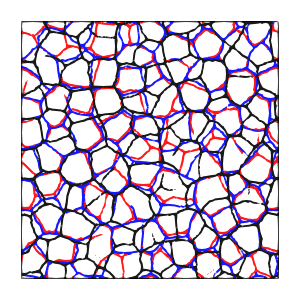
\includegraphics[width=\textwidth]{Chapter4/figures/2D/psic_constant.png}
    \caption{}
    \label{fig: Chapter4/2D/morphology_psic_constant}
  \end{subfigure}
  \begin{subfigure}[b]{0.4\textwidth}
    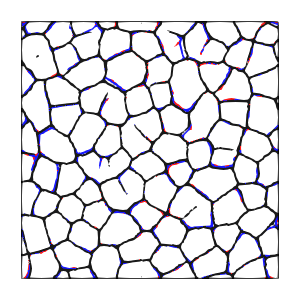
\includegraphics[width=\textwidth]{Chapter4/figures/2D/Gc_constant.png}
    \caption{}
    \label{fig: Chapter4/2D/morphology_Gc_constant}
  \end{subfigure}
  \begin{subfigure}[b]{0.1\textwidth}
    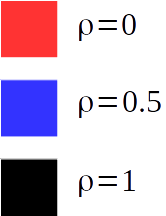
\includegraphics[width=\textwidth]{Chapter4/figures/rho.png}
    \caption*{}
    \vspace{0.75in}
  \end{subfigure}
  \caption{ Superposition of fracture networks obtained by three samples of different coefficients of correlation, using the PSE kernel. Only the volume within the damage contour of $d = 0.9$ is shown to represent the resulting fracture network. Three samples are sampled (a) by holding $\Gc$ constant and (b) by holding $\psi_c$ constant. }
  \label{fig: Chapter4/2D/compare_morphology}
\end{figure}
